\documentclass[runningheads]{llncs}
\usepackage{graphicx}
\usepackage[colorlinks]{hyperref}
\hypersetup{
    colorlinks = false,
    linkbordercolor = {blue}
}
\usepackage{listings}
\usepackage{courier}
\renewcommand{\floatpagefraction}{.8}
%
\begin{document}

\title{ShabbyPages: A Recipe for Repeatable, Synthetic, Modern Document Images}
%\author{Alexander Groleau\inst{1,2} \and
%  Kok Wei Chee\inst{1} \and
%  Stefan Larson\inst{3} \and
%  Jonathan Boarman\inst{1} \and
%  Samay Maini\inst{1}}
%
%\authorrunning{A. Groleau et al.}
%
%\institute{Sparkfish LLC (\email{augraphy@sparkfish.com})
%  \and
%  Left Associates LLC (\email{research@left.associates})
%  \and
%  Vanderbilt University}

\author{Anonymous ICDAR 2023 submission}

\maketitle

\begin{abstract}
The ShabbyPages document image dataset is produced using the Augraphy document image augmentation tool.
The development of the computation pipeline used to generate the corpus is discussed, and the results presented.
The final corpus contains over 6000 "born-digital" ground truth document images, sourced on the Web, with synthetically-noised counterparts (``shabby pages'') that appear to have been printed and faxed, photocopied, or otherwise altered through physical processes.
The release of this dataset and the recipe for its production attempts to address a growing need for labeled training document images for supervised learning tasks.
The results of several experiments are discussed, in which the corpus trains performant convolutional denoisers, which remove real noise features with a high degree of human-perceptible fidelity, establishing baseline performance for a new ShabbyPages benchmark.
\end{abstract}

\section{Introduction}
Supervised learning requires a collection of training data and accompanying ``labels'', which in the graphical modality are clean images, free of noise or other degradations.
ShabbyPages is a large dataset composed of 6202 clean/noisy pairs of images taken from 600 digital documents.
Information about the set's contents and its relation to other datasets are explored in the next section.
The noisy images were created from their clean origins by the application of a pipeline developed with the Augraphy library; the production of ShabbyPages is detailed in the third section, with all source code and input materials made openly available.
The final dataset is used to train several denoising models which are compared directly and whose prediction results are compared together in the final section.

\section{The Dataset}
ShabbyPages joins a rapidly growing number of open-source datasets freely available online.
Human activity today generates a tremendous amount of data, with many people choosing to publish theirs on websites like Kaggle \cite{ref_Kaggle}, Hugging Face Hub \cite{ref_HuggingFaceHub}, and many more.
All of this data is arranged into categories: sets exist which contain text, images, audio, and data from other modalities, with each set often collected and designed for a purpose.
Of the many image datasets available, the authors understand few to have been designed for groundtruthed supervised learning of document-specific tasks like binarization or denoising.
In fact, we could find only one other set compiled for doing so with images of \textit{modern} documents: NoisyOffice \cite{ref_NoisyOffice}.

\begin{figure}
\centering
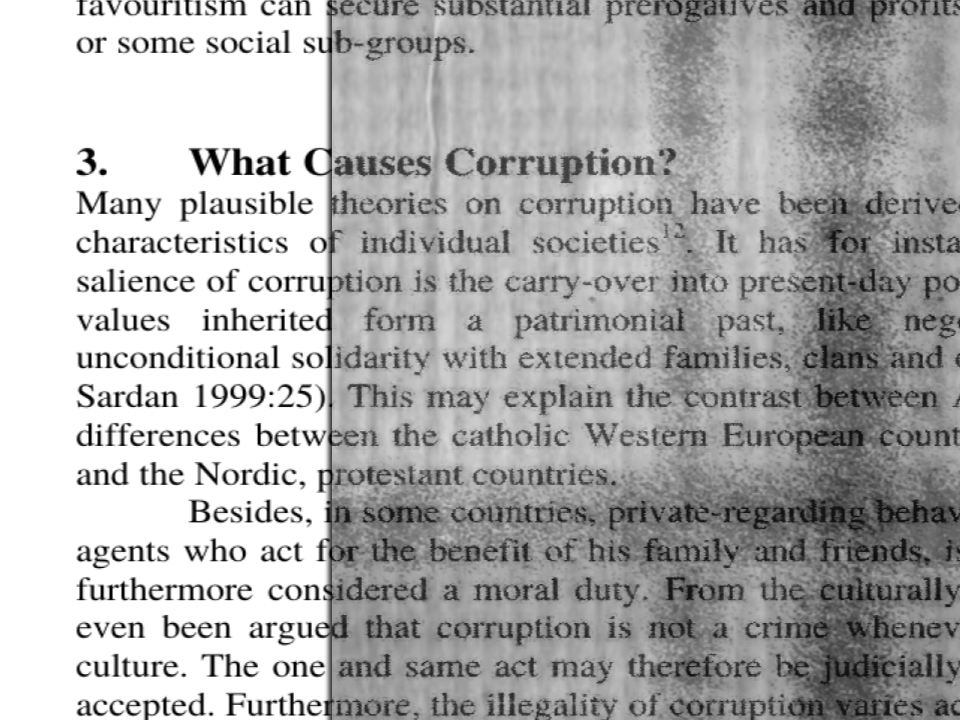
\includegraphics[width=0.98\columnwidth, frame]{Article_Hero_Picture_Shadow.png}
\caption{Example ShabbyPages image, before (left side) and after augmentationi (right side).} \label{fig1}
\end{figure}

\subsection{Features}
Modern artificial neural networks produce a latent representation of their training data, a space from which outputs are sampled.
In deep networks, these representations live within multiple layers, each of which corresponds to a feature of the input data.
Document images are a particularly interesting category, as the data within the documents each picture represents is itself frequently multi-modal; the document may contain an image and its description, a table with statistics, multiple regions of structured and formatted text, and even other documents, making their internal representations by neural networks often quite complicated.

Networks with a wider variety of latent representations frequently perform better when generalizing their learned functions to other tasks.
Procuring a large-enough volume of robust-enough training data is paramount.
Several sets of such images exist, many intended for processing by deep neural nets; Table 1 below contains a comparison of some of the key hyperproperties of the ShabbyPages set compared with other popular document image datasets.

\textbf{Diversity.} We use the diversity metric as defined in \cite{kang-etal-2018-data,larson-etal-2019-outlier} to help us measure how diverse a dataset is.
This metric is defined as 
$$
Diversity(X) = \frac{1}{|X|^2} \sum_{a\in X} \sum_{b\in X} \|f(a)-f(b)\|_2
$$
where $f(\cdot)$ is an embedding function mapping the input image into an \emph{n}-dimensional vector space.
Here, we use CLIP's ViT model \cite{clip}, which embeds each image into a 512-dimensional embedding space.
The intuition behind the diversity metric is that datasets where images are highly similar will have lower diversity scores, and datasets where images share less visual similarity will have higher diversity scores.
A dataset with low diversity might not be representative enough of the real world, and low diversity may often correlate with task easiness.

\begin{table}
\centering
\caption{Document Image Dataset Feature Comparison}\label{tab1}
\begin{tabular}{|@{\hspace{1em}}l@{\qquad}|@{\hspace{1em}}l@{\qquad}|@{\hspace{1em}}l@{\qquad}|@{\hspace{1em}}l@{\qquad}|@{\hspace{1em}}l@{\qquad}|}
\hline
Feature & ShabbyPages & NoisyOffice & RVL-CDIP & Tobacco800 \\
\hline
Images & 6202 & 72 & 400000 & 1290\\
Diversity & 0.488 & 0.317 & & \\
Document-specific & Yes & Yes & Yes & Yes\\
Synthetic & Yes & Yes & No & No\\
Groundtruthed? & Yes & Yes & No & No\\
Font size & Multiple & 16pt & Multiple & Multiple\\
Paper styles & Multiple & 1 & Multiple & Multiple\\
Multilingual & Yes & No & No & No\\
Documents contain images? & Yes & No & Yes & Yes\\
Pre-categorized & No & No & Yes & Yes\\
\hline
\end{tabular}
\end{table}

\subsubsection{NoisyOffice}
The NoisyOffice database \cite{ref_NoisyOffice} contains a very low 4 base images, 2 types of font, 3 font sizes, and 4 types of noise, for a total of 72 unique images.
The groundtruth images were produced in a standard word processor, with the simulated noisy images produced by first adding noise to a blank sheet of paper, storing that as a background image after digital scanning, then overlaying the foreground text onto the noisy background texture.
An additional set of real NoisyOffice images was produced, where the foreground text was printed on blank white sheets, the results of which were physically augmented by the introduction of footprints, coffee stains, wrinkles, and folds.

ShabbyPages began with 600 documents sourced from the Internet from culturally-important sources.
A manifest is included in the dataset which contains an ordered table of the filenames, the languages present in the document, the download URL for the file, and an English name or acronym for the source organization or person.
These documents were split into their constituent pages, which were then passed through an Augraphy pipeline we tuned over a month or two.
This tuning amounted to tweaking numerical parameters for each of the 24 different augmentations from the Augraphy library.
All or none of these may have applied to each input image, and only one pipeline run was completed per image.
Each augmentation has a high degree of internal variability due to several calls to a pseudorandom number generator on which several transforms depend.
The conjunction of all these factors implies ShabbyPages is a sample from a massive space.
Indeed, the cosine similarity computed over OpenAI's CLIP representations of each output image averages to 0.49, much higher than NoisyOffice's 0.31.
Augraphy does not yet have augmentations for footprints or coffee stains, so the dark regions and edges of the stains and prints were simulated with features introduced by other augmentations, but Augraphy does contain the PaperFactory transformation which selects and crops a texture from a local directory of paper images.
The result of a PaperFactory application is the foreground text ``printed'' onto the background texture, similar to NoisyOffice's construction.

\subsection{RVL-CDIP}
The RVL-CDIP dataset \cite{ref_RVL-CDIP} consists of 400,000 grayscale images divided into 16 document classes, each with a similar number of elements.
The dataset is pre-segmented into 320,000 training, 40,000 test, and 40,000 validation images, facilitating immediate use in machine learning applications.
The classes represented are the following:

\begin{center}
letter, form, email, handwritten, advertisement, scientific report,
scientific publication, specification, file folder, news article,
budget, invoice, presentation, questionnaire, resume, memo.
\end{center}

The images exhibit poor fidelity with what we can imagine their originals to have been, contain substantial noise, and many were scanned at around 100 pixels per inch, quite a low resolution for documents.
None of the images in the CDIP set come with groundtruths.

The collection of RVL-CDIP is an impressive feat in its own right: nearly half a million scanned documents with real noise, already categorized.
Augraphy makes synthetic documents, intended to simulate real noise without the need to physically produce it.
One of the augmentations used in the ShabbyPages set is BadPhotoCopy, which mimics low-fidelity noisy or damaged scans.

\subsection{Tobacco800}
Tobacco800, like RVL-CDIP, is a subset of the Complex Document Image Processing collection, containing images of documents originally internal to tobacco companies, and released under the Tobacco Master Settlement Agreement.
The corpus is composed of 1290 images, gathered and scanned at different times and by different devices.
Several of the images in this set are consecutively-numbered pages, increasing the set's utility for certain image analysis tasks \cite{ref_Tobacco800}.
Document images in this set vary from from 150 to 300 DPI with dimensions between 1200 pixels wide and 2500 pixels tall on the low end and 1600 by 3200 on the high.

Every document in the ShabbyPages groundtruth set is a multi-page document.
The released set was exported at 150 DPI, but the original documents are also distributed, so re-exporting at a higher resolution is trivial.
The smallest image is 532 by 532, with the largest 3336 wide by 12157 tall.
6202 images are present in ShabbyPages, but this number could easily be increased by simply running another Augraphy pipeline to generate more.

\subsection{ShabbyPages Compared}
Supervised learning tasks require labeled training data, called the ground truth.
Much of the world's data does not come with labels, which instead must be created by humans in some fashion.
In Table 1, we indicated that NoisyOffice was the only other groundtruthed dataset we examined.
This isn't strictly true: there are projects to add some types of groundtruth to RVL-CDIP \cite{ref_zenodo,ref_goldmann} and Tobacco800 \cite{ref_tobacco800gt2,ref_tobacco800gt1}, but the images in these sets were produced by real scans, without an accompanying original digital document.
Conversely, NoisyOffice contains images of real scanned documents intended for validation, as well as their digital groundtruth and synthetic training image data.

ShabbyPages includes not only the groundtruth images, but also the original digital documents used to produce them, and the software for fully reproducing the ShabbyPages set, allowing anyone to quickly produce a new set in the Shabby family, optionally re-exporting groundtruths at a different resolution beforehand.
The 6202 images in the ShabbyPages release set are really just the first sample from the space of these documents; we encourage building your own.
NoisyOffice is the only other set we examined that contains its digital provenance, but the released database materials lack a means of reproducing the simulated printing method used to create the NoisyOffice training data.
Augraphy's PaperFactory augmentation is such a tool.
The other sets are not even theoretically extensible in this way.


\subsection{Statistics}
ShabbyPages contains documents from multiple classes, which contain many types of information.

Table 2 below contains some statistics for the dataset, in grayscale, at a standard resolution of 150 ppi.

\begin{table}
    \centering
    \caption{ShabbyPages dataset statistics.}\label{tab1}
    \begin{tabular}{@{\hspace{2em}}l@{\qquad}@{\hspace{2em}}l@{\qquad}}
        \toprule
        \textbf{Statistic} & \textbf{Value} \\
        \midrule
        Num. Images & 6202 \\
        DPI & 150 \\
        Max image size & --- \\
    \bottomrule
    \end{tabular}
\end{table}

\subsection{Limitations}
The ShabbyPages collection is a comprehensive entrant to the public datasphere, but with a relatively low starting document volume, makes some important omissions.

First, we arbitrarily selected 600 as the number of source documents.
The number of final images of pages depends on this, and so is similarly arbitrary.

There are only a few languages represented, which reflects a number of biases, including the following:
\begin{itemize}
\item The native languages of the document-searchers
\item The locations from which the document-searchers searched
\item The search techniques used by each document-searcher
\end{itemize}

This work does not account for them, but these biases are significant determiners on the set of input documents.
We hoped to overcome this somewhat by picking a suitably large number of input documents, and settled at 600.

\section{Construction}
This section describes the dataset generation methodology; code for all of this is available on GitHub.

\subsection{Data Gathering}
A team of workers searched the public internet for PDFs of many different kinds.
600 unique documents were retrieved, totaling 6202 pages.
A similar process was completed to collect paper textures on which to "print" the documents: 300 unique textures were gathered, all of which are either in the public domain or carry CC-0, CC-BY, or CC-BY-SA licenses.
Care was taken to retrieve freely-available and attributable documents; a CSV file containing document and paper texture links (as of time of download), with their sources, is available and distributed with the dataset.
We also manually reviewed the gathered documents to verify that no personal identity information was present within the corpus.

\subsection{PDF to PNG}
The ~pdftoppm~ tool from the ~poppler-utils~ package was used to split the PDF documents into individual pages.
Each page was converted to a PNG image at 150dpi, a common printing resolution.
Because the majority of these documents were created with the standard US Letter dimensions, this resulted in the most common image dimension being 1275 pixels wide by 1650 pixels tall.

\begin{lstlisting}[language=bash]
  pdftoppm document_name.pdf document_name -png -r 150
\end{lstlisting}

\subsection{Developing the Pipeline}
The Augraphy library presents an easy-to-use API for constructing feature pipelines, which has been designed for interoperability with other augmentation tools, and within the broader data ecosystem.
While Augraphy's default pipeline has what we believe to be quite realistic defaults, we wanted a broader range of features from this dataset than those the default pipeline could produce.
To address this, we broke all of the parameters for every augmentation constructor out into separate variables, tweaking these and committing the new pipeline to GitHub.
We created an automated daily build in GitHub Actions to render a random selection of ground-truth images with the updated pipeline, then our team met frequently to discuss the output and make adjustments to the pipeline.

\subsection{Processing Augraphy on a multicore system}
Execution time is dependent on which augmentations are executed at runtime; an Augraphy pipeline can take several seconds to process large images.
The library is under active development with performance enhancements underway, but the time cost to generate large datasets sequentially is prohibitive when dealing with thousands of files, so we use a multi-process pooling technique to distribute the workload across many processor execution threads.
For each process, we generate a new pipeline, run the pipeline object on an image, and save the output, using the code below:

\begin{lstlisting}[language=Python]
    import os
    import cv2
    from multiprocessing import Pool
    from pathlib import Path

    input_path = Path("/path/to/input/images")
    filenames = [(input_path / name)
      for name
      in os.listdir(input_path)]

    pool = Pool(os.cpu_count())

    def run_pipeline(filename):
        image = cv2.imread(filename)
        # returns the current Shabby Pages pipeline
        pipeline = get_pipeline()
        data = pipeline.augment(image)
        shabby_image = data["output"]
        cv2.imwrite(filename.parent / f"{filename.stem}-shabby{filename.suffix}")

    pool.map(run_pipeline, filenames)

\end{lstlisting}

Processing all 6202 images took less than half an hour on the 64 cores of a Graviton3 c7g.16xlarge instance on AWS.

\section{Experimentation with the ShabbyPages Set}
Binarization and denoising are two important techniques for the removal of unwanted data from images.
Both approaches can be achieved by supervised learning of relationships between features of the input and output data.
In this section, we train and compare several instances of the NAFNet \cite{ref_nafnet} architecture as denoisers and binarizers, and evaluate these models' predictions on both the NoisyOffice and ShabbyPages datasets.
The model was ``off-the-shelf''; besides rigging up the training inputs, we made no alterations to the 

\subsection{Motivation for Denoising}
Digital computation has enabled humanity to produce ever-growing amounts of both data and reasons to process it.
Doing so is easiest when the data is free of unexpected outliers, the signal has less jitter, or when our aesthetic sensibilities aren't injured.

\subsection{Binarization}
In this section, we discuss results obtained by training a binarizing denoiser to both restore augmented images to their ground truths and to classify pixels as foreground.

We first performed an ensemble binarization preprocessing step on the clean groundtruth images.
For each image, we computed the Niblack, Sauvola, and Otsu thresholds, using these to binarize three copies of the input. The average over the resulting matrices was taken elementwise, producing the final binarized groundtruth.

One instance of the model was trained on the SimulatedNoisyOffice corpus, while the other was trained on a subset of ShabbyPages, in both cases using the relevant ensemble-binarized groundtruths.
As a test, these models were used to denoise and binarize both the NoisyOfficeReal dataset and a testing subset taken from ShabbyPages which does not overlap the training subset.
Common image processing metrics were applied to the predictions made by each model, comparing these to the (preprocessed) groundtruths.
The averages of each metric over all such predictions was taken; these are presented in Table 2.

\begin{table}[]
    \centering
    \caption{Document image binarization performance of a NAFNet model trained and tested on ShabbyPages and NoisyOffice.}
    %\caption{Document image binarization performance between NoisyOffice-trained and ShabbyPages-trained NAFNet binarizing de    noisers on cross-validation task}
    \scalebox{0.9}{
    \begin{tabular}{lllll}
    \toprule
    \textbf{Training Set~~} & \textbf{Test Set} & \textbf{SSIM$\uparrow$~} & \textbf{RMSE$\downarrow$~} & \textbf{PSNR$\uparrow$} \\
        \midrule
        \textsf{ShabbyPages} & \textsf{ShabbyPages} & 0.926 & 2.99 & 39.3\\
        \textsf{NoisyOffice-sim} & \textsf{NoisyOffice-real~} & 0.987 & 3.80 & 36.7\\
        \textsf{ShabbyPages} & \textsf{NoisyOffice-real} & 0.947 & 3.20 & 38.1\\
        \textsf{NoisyOffice-sim} & \textsf{ShabbyPages} & 0.811 & 5.38 & 34.6\\
        \bottomrule
    \end{tabular}}
    \label{tab:binarization_results}
\end{table}

\subsubsection{Interpretation}
As a baseline, we first evaluated the models against test sets associated with their training databases; the model trained on SimulatedNoisyOffice was used to enhance the RealNoisyOffice set, while the ShabbyPages-trained model cleaned a testing subset drawn from the full ShabbyPages set.

We considered three common image processing metrics: structural similarity index, root mean squared error, and peak signal-to-noise ratio.

Although the ShabbyPages-trained NAFNet predicted cleaned ShabbyPages images with a lower structural similarity score than the NoisyOffice-trained model predicted cleaned RealNoisyOffice images, the ShabbyPages model achieved superior performance on RMSE and PSNR.
The ShabbyPages corpus contains a much higher feature diversity than NoisyOffice, so the lower SSIM score was not unexpected; local relationships between pixels were easier to encode for the NoisyOffice model, possibly because there are simply fewer relationships.
The RMSE and PSNR results on the other hand indicate that the ShabbyPages-trained model learned to remove more noise with higher fidelity, and more accurately predicted foreground pixels than the NoisyOffice model.
This discrepancy can partly be explained by the RealNoisyOffice corpus having been physically-noised as opposed to ShabbyPages' purely synthetic noise; small-scale features in the RealNoisyOffice testing data are not quite identical to the SimulatedNoisyOffice training inputs, while both the training and testing data taken from ShabbyPages was constructed by the same means.
In the latter case, the \textit{diversity} of the ShabbyPages data is much higher (TODO: add diversity score info), and this instance of the NAFNet may have been able to generalize over noise types better than the NoisyOffice-trained network with its lower training diversity.

The second stage of the binarization experiment was to cross-validate these models by predicting cleaned images using the other testing set as inputs.
Here, the ShabbyPages-trained model achieved all-around better performance than the NoisyOffice-trained model, with a much higher structural similarity score (0.947 vs. 0.811), lower RMSE, and higher PSNR.
This is a strong indicator that neural networks trained on ShabbyPages can outperform those trained on NoisyOffice when generalizing to other datasets.

Interestingly, the NoisyOffice-trained model RMSE and PSNR scores were lower when cleaning RealNoisyOffice than the Shabby-trained model: we were able to achieve a 3.5 decibel improvement in peak signal-to-noise ratio over the SimulatedNoisyOffice-trained model.


%
% ---- Bibliography ----
%
% BibTeX users should specify bibliography style 'splncs04'.
% References will then be sorted and formatted in the correct style.
%
 \bibliographystyle{splncs04}
 \bibliography{paper}

%\begin{thebibliography}{8}
%\bibitem{ref_Kaggle}
%  https://www.kaggle.com/datasets
%\bibitem{ref_HuggingFaceHub}
%  {https://huggingface.co/datasets}
%\bibitem{ref_RDCL2019}
%{Christian Clausner, RDCL2019 Competition Dataset (Recognition of Documents with Complex Layouts) (RDCL2019) ,1,ID:RDCL2019\_1,URL:https://tc11.cvc.uab.es/datasets/RDCL2019_1}
%
%\bibitem{ref_Tobacco800}
%{David Doermann, Tobacco 800 Dataset (Tobacco800) ,1,ID:Tobacco800_1,URL:https://tc11.cvc.uab.es/datasets/Tobacco800_1}
%
%\bibitem{ref_icdar}
%{Harold Mouchère, ICDAR 2019 Competition on Recognition of Handwritten Mathematical Expressions and Typeset Formula Detection (ICDAR2019-CROHME-TDF) ,1,ID:ICDAR2019-CROHME-TDF\_1,URL:https://tc11.cvc.uab.es/datasets/ICDAR2019-CROHME-TDF_1}
%
%\bibitem{ref_NoisyOffice}
%{Castro-Bleda, MJ.; España Boquera, S.; Pastor Pellicer, J.; Zamora Martínez, FJ. (2020). The NoisyOffice Database: A Corpus To Train Supervised Machine Learning Filters For Image Processing. The Computer Journal. 63(11):1658-1667. https://doi.org/10.1093/comjnl/bxz098}
%
%\bibitem{ref_RVL-CDIP}
%  @article{DBLP:journals/corr/HarleyUD15,
%  author    = {Adam W. Harley and
%               Alex Ufkes and
%               Konstantinos G. Derpanis},
%  title     = {Evaluation of Deep Convolutional Nets for Document Image Classification
%               and Retrieval},
%  journal   = {CoRR},
%  volume    = {abs/1502.07058},
%  year      = {2015},
%  url       = {http://arxiv.org/abs/1502.07058},
%  eprinttype = {arXiv},
%  eprint    = {1502.07058},
%  timestamp = {Mon, 13 Aug 2018 16:48:54 +0200},
%  biburl    = {https://dblp.org/rec/journals/corr/HarleyUD15.bib},
%  bibsource = {dblp computer science bibliography, https://dblp.org}
%}
%
%\bibitem{ref_NoisyOfficeDatabase}
%{F. Zamora-Martinez, S. España-Boquera and M. J. Castro-Bleda, Behaviour-based Clustering of Neural Networks applied to Document Enhancement, in: Computational and Ambient Intelligence, pages 144-151, Springer, 2007.}
%
%\bibitem{ref_UCIMLR}
%{Dua, D. and Graff, C. (2019). UCI Machine Learning Repository [http://archive.ics.uci.edu/ml]. Irvine, CA: University of California, School of Information and Computer Science.}
%
%\bibitem{ref_DocCreator}
%  {Journet Nicholas, Visani Muriel, Mansencal Boris, Van-Cuong Kieu, Billy Antoine, DocCreator: A New Software for Creating Synthetic Ground-Truthed Document Images. J. Imaging 2017, 3, 62.}
%\bibitem{ref_goldmann}
%  {Pau Riba, Anjan Dutta, Lutz Goldmann, Alicia Fornes, Oriol Ramos, Josep LLados: "Table Detection in Invoice Documents by Graph Neural Networks", ICDAR, 2019.}
%\bibitem{ref_zenodo}
%  {Layout Analysis Groundtruth for the RVL-CDIP Dataset. Goldmann, Lutz. 10.5281/zenodo.3257319}
%\bibitem{ref_tobacco800gt1}
%  {Guangyu Zhu, Yefeng Zheng, David Doermann,and Stefan Jaeger. Multi-scale Structural Saliency for Signature Detection. In Proc. IEEE Conf. Computer Vision and Pattern Recognition (CVPR 2007), pp. 1‐8, 2007.}
%\bibitem{ref_tobacco800gt2}
%  {Guangyu Zhu and David Doermann. Automatic Document Logo Detection. In Proc. 9th Int. Conf. Document Analysis and Recognition (ICDAR 2007), pp. 864‐868, 2007.}
%
%\bibitem{ref_NAFNet}
%  @misc{https://doi.org/10.48550/arxiv.2204.04676,
%  doi = {10.48550/ARXIV.2204.04676},
%  url = {https://arxiv.org/abs/2204.04676},
%  author = {Chen, Liangyu and Chu, Xiaojie and Zhang, Xiangyu and Sun, Jian},
%  keywords = {Computer Vision and Pattern Recognition (cs.CV), FOS: Computer and information sciences, FOS: Computer and information sciences},
%  title = {Simple Baselines for Image Restoration},
%  publisher = {arXiv},
%  year = {2022},
%  copyright = {arXiv.org perpetual, non-exclusive license}
%}
%
%
%\end{thebibliography}
\end{document}

